\documentclass[byrevtex,amssymb,aps,pra,floatfix,letterpaper]{revtex4}
\usepackage{graphicx}
\usepackage{hyperref}
\bibliographystyle{apsrev}
\date{\today}
\pagestyle{plain}
\newcommand{\degree}[0]{$^\circ$}

\begin{document}

\title{Experiment 1: Excited-state properties of 2-naphthol (the acidity constants)}

\date{\today}

\maketitle

\section{Introduction}

The electronic structure of a molecule determines such physical and chemical properties as its charge distribution, geometry (and therefore the dipole moment), ionization potential, electron affinity, and of course, chemical reactivity. If the electronic structure of a molecule were to be changed, one would expect its physical and chemical properties to be altered. Such a rearrangement can occur when a molecule is raised to an electronically excited state via the absorption of a quantum of light (i.e., a photon) whose energy matches the energy gap between the ground and excited states.

For most organic molecules that contain an even number of electrons, the ground state is characterized by having all electron spins paired; the net spin angular momentum is zero, and such an arrangement is called a singlet state. When considered in terms of molecular orbitals (MOs), electronic excitation involves the promotion of an electron from a filled MO to a higher, unoccupied MO. This new electronic configuration, which characterizes the electronically excited state, may be one in which the two electrons reside in the singly occupied MO's with opposite spins. Accordingly, this electronically excited state is also a singlet. The ground, and lowest electronically excited, singlet states are often denoted as S$_0$ and S$_1$, respectively. Higher excited singlet states are referred to
as S$_2$, S$_3$, ..., S$_n$.

Although measurements of the physical and chemical properties of a molecule in its ground state can be carried out, more or less, at leisure (assuming that the molecule is thermally stable), the examination of these properties in its excited states is severely hampered by the fact that these states are very short-lived. For most molecules, S$_1$ states have lifetimes ranging from 10$^{-6}$ -- 10$^{-11}$ s (i.e., $\mu$s to some ps). Excited states are metastable; they undergo decay processes that dissipate the energy they possess relative to more stable products. For example, the excited state of a molecule may, in general: spontaneously return (spontaneous emission; lifetime 10$^{-6}$ to 10$^{-9}$ s) to the ground state via photon emission (fluorescence), convert electronic excitation into vibrational energy (eventually generating heat), undergo bond dissociation or rearrangement (``fast'') or a change in electron spin multiplicity (``slow''). Because spontaneous emission from an excited state (i.e., fluorescence) often takes place very rapidly, fluorescence can be used as a probe, or measurement, of excited state concentration (i.e., fluorescence assay). In addition, fluorescence studies can provide information about the physical and chemical properties of these short-lived singlet states. This field of experimentation is called photochemistry or photophysics depending on what is being studied. In this experiment, the ground and excited state acidity constants of 2-naphthol (ArOH; see Fig. \ref{fig1}) will be determined. For more information on optical spectroscopy, see Refs. \cite{ATKINS1, SILBEY, CHANG}.

\begin{figure}[!htp]
\begin{center}
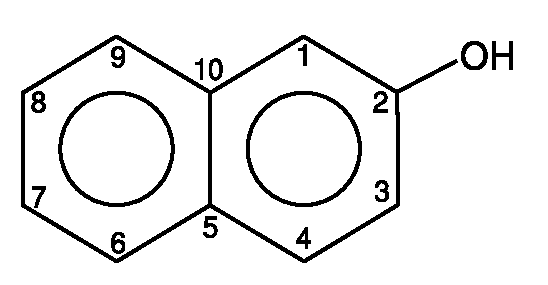
\includegraphics[scale=0.5]{fig1}
\caption{Structure of 2-naphthol (ArOH). Also called $\beta$-naphthol.}
\label{fig1}
\end{center}
\end{figure}

\section{Theory}

In aqueous solution, ArOH behaves as a weak acid, forming the hydronium ion and its conjugate base, the naphthoxy anion, ArO$^-$:

\begin{equation}
\label{eq1}
\textnormal{ArOH} + \textnormal{H}_2\textnormal{O} \rightleftharpoons \textnormal{H}_3\textnormal{O}^+
+ \textnormal{ArO}^-
\end{equation}

\noindent
It is instructive to measure the acidity constant of ArOH in its lowest excited electronic state, denoted as $K^*_a$, and to compare this value with that of the ground state $K_a$. This information indicates how the change in electron structure alters the charge density at the oxygen atom. The experimental method is best introduced in terms of the energy-level diagram shown in Fig. \ref{fig2}.

\begin{figure}[!htp]
\begin{center}
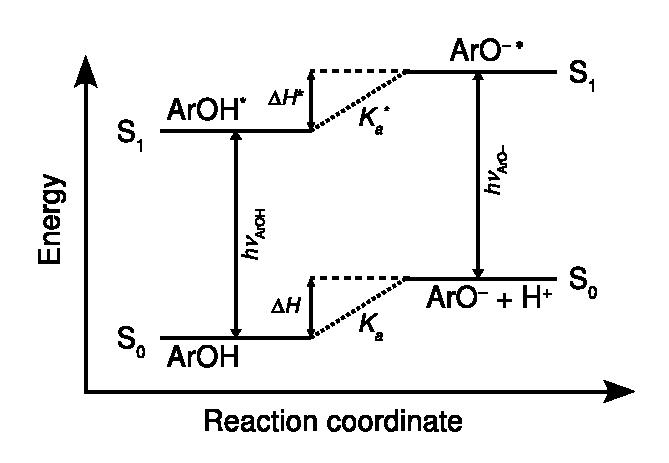
\includegraphics[scale=0.8]{fig2}
\caption{A schematic diagram of the ground (S$_0$) and first excited singlet state (S$_1$) energies of free naphthol and its conjugate base, the naphthoxy anion, in aqueous solution. For transitions shown, the up arrow indicates absorption and down arrow fluorescence.}
\label{fig2}
\end{center}
\end{figure}

The relative energies of the free acid and its conjugate base (i.e., the naphthoxy anion) are indicated for both the electronic ground (S$_0$) and lowest excited (S$_1$) states in aqueous solution (see Fig. \ref{fig2}). Each anion is elevated with respect to its free acid by an energy, $\Delta H$ and $\Delta H^*$, respectively. These are the enthalpies of deprotonation. Both the ground state acid and its conjugate base can be transformed to their respective excited states via the absorption of photons of energy $h\nu_\textnormal{\tiny ArOH}$ and $h\nu_{\textnormal{\tiny ArO}^-}$. For simplicity, these absorptive transitions in Fig. \ref{fig2} are shown to be equal to the fluorescence from the excited to the ground states of the acid and conjugate base. Note that the ground and excited state vibrational levels that are involved in the transitions are not indicated.

The free energy of deprotonation of ArOH can be expressed in terms of the enthalpy and entropy of deprotonation, and the equilibrium (ionization) constant:

\begin{eqnarray}
\label{eq2}
& & \Delta G = \Delta H - T\Delta S = -RT\ln(K_a)\textnormal{ \hspace{1cm}(for the ground state)}\\
\nonumber
& & \Delta G^* = \Delta H^* - T\Delta S^* = -RT\ln(K_a^*)\textnormal{ \hspace{0.5cm}(for the excited state)}
\end{eqnarray}

\noindent
for the S$_0$ and S$_1$ states, respectively. If we make the assumption that the entropies of dissociation of ArOH and ArOH$^*$ are equal, it follows that

\begin{equation}
\label{eq3}
\Delta G - \Delta G^* \approx \Delta H - \Delta H^* = -RT\ln\left(\frac{K_a}{K_a^*}\right)
\end{equation}

\noindent
and thus from Fig. \ref{fig2}, using a Hess' law approach (i.e., by considering a closed loop consisting of the absorption, deprotonation in excited state, emission, and protonation in the ground state), it can be deduced that

\begin{eqnarray}
\label{eq4}
& & N_Ah\nu_\textnormal{\tiny ArOH} + \Delta H^* - N_Ah\nu_{\textnormal{\tiny ArO}^-} - \Delta H = 0\\
\nonumber
& & \Rightarrow \Delta H - \Delta H^* = N_A\left(h\nu_\textnormal{\tiny ArOH} - h\nu_{\textnormal{\tiny ArO}^-}\right)
\end{eqnarray}

\noindent
where $h$ is Planck's constant and $\nu$'s are the transition frequencies (Hz). Avogadro's number, $N_A$, has been included to put each energy term on a molar basis. Combining Eqs. (\ref{eq3}) and (\ref{eq4}) and rearranging gives

\begin{equation}
\label{eq5}
\ln\left(\frac{K_a}{K_a^*}\right) = \frac{hN_A\left(\nu_{\textnormal{\tiny ArO}^-} - \nu_\textnormal{\tiny ArOH}\right)}{RT}
\end{equation}

\noindent
Thus knowledge of the energy gap between the ground and first excited states for both the free acid and its conjugate base leads to an estimate for $K_a^*$, if $K_a$ is known. The analysis presented above, which accounts for the observed thermodynamic and spectroscopic energy differences, was first developed by F\"orster \cite{FORSTER}. This approach is thus often referred to as a F\"orster cycle. Eq. (\ref{eq5}) can be recast into the following form:

\begin{eqnarray}
\label{eq6}
& & \ln\left(\frac{K_a}{K_a^*}\right) = \frac{\log\left(\frac{K_a}{K_a^*}\right)}{\log(e)}\approx 2.303\log\left(\frac{K_a}{K_a^*}\right) = 2.303\left(\log(K_a) - \log(K_a^*)\right)\\
\nonumber
& & \textnormal{Recall that }pK_a = -\log(K_a)\textnormal{ and }pK_a^* = -\log(K_a^*).\\
\nonumber
& & \Rightarrow \ln\left(\frac{K_a}{K_a^*}\right) = 2.303\left(pK_a^* - pK_a\right)\\
\nonumber
& & \Rightarrow pK_a^* = pK_a - \frac{N_Ah\left(\nu_\textnormal{\tiny ArOH} - \nu_{\textnormal{\tiny ArO}^-}\right)}{2.303RT}
= pK_a - \frac{N_Ahc\left(\tilde{\nu}_\textnormal{\tiny ArOH} - \tilde{\nu}_{\textnormal{\tiny ArO}^-}\right)}{2.303RT}
= pK_a - \frac{N_Ahc\Delta\tilde{\nu}}{2.303RT}
\end{eqnarray}

\noindent
where $c$, the speed of light (2.9979 $\times$ 10$^8$ m/s), has been incorporated in the expression to convert the transition frequencies of ArOH and ArO$^-$ into wavenumbers (m$^{-1}$, $\tilde{\nu}$ -- use of $\tilde{}$ only signifies the use of wavenumber units -- typically expressed as cm$^{-1}$ but must be entered as m$^{-1}$ when using SI units!), a common spectroscopic energy unit. Furthermore $h$ is the Planck's constant (6.626076 $\times$ 10$^{-34}$ Js), $N_A$ is Avagadro's constant (6.022137 $\times$ 10$^{23}$ mol$^{-1}$), $R$ is the ideal gas constant (8.31451 J mol$^{-1}$ K$^{-1}$), and $T$ is the temperature (K; here room temperature). In the last stage, the acidity constants are expressed as $pK$ values, where $pK_a = -\log(K_a)$. Note that here $\ln$ stands for natural base logarithm while $\log$ refers to base ten logarithm.

\begin{figure}[!htp]
\begin{center}
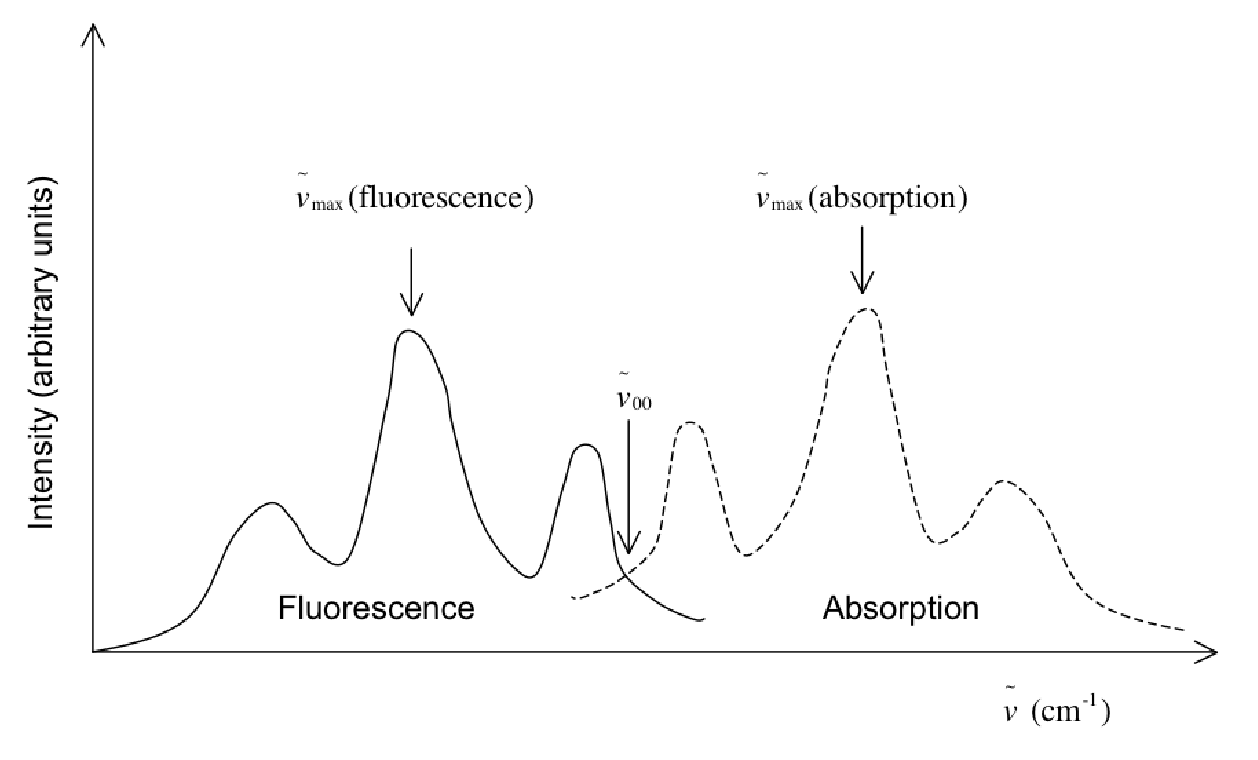
\includegraphics[scale=0.5]{fig3}
\caption{A schematic diagram of the absorption and fluorescence spectra of a molecule. It is assumed that these transitions are between the same two electronic states, i.e., S$_0$ $\leftrightarrow$ S$_1$. Here $\tilde{\nu}_{00}$ marks the ``0-0 transition'' and it is obtained from the crossing point of the spectra. In the present case $\tilde{\nu}_{00}$ would correspond to $\tilde{\nu}_\textnormal{\tiny ArOH}$ or $\tilde{\nu}_{\textnormal{\tiny ArO}^-}$.}
\label{fig3}
\end{center}
\end{figure}

\section{Absorption and fluorescence spectroscopy}

The question now is how to obtain the spectroscopic energy difference ($\Delta\tilde{\nu}$ in Eq. (\ref{eq6})) pertinent to the F\"orster cycle in 2-naphthol. This difference depends on both $\nu_\textnormal{\tiny ArOH}$ and $\nu_{\textnormal{\tiny ArO}^-}$, which have to be determined experimentally. In general there are three different ways to do this:

\begin{enumerate}

\item Measure UV/VIS absorption spectra for both ArOH and ArO$^-$ and obtain $\Delta\tilde{v}$ approximately from the absorption maxima of the species. To be exact, one would have to locate the pure electronic transitions that are not accompanied with molecular vibrations (``0-0 transitions''; often denoted by $\tilde{v}_{00}$). These are usually difficult to locate exactly from the UV/VIS absorption spectra.

\item Measure fluorescence emission spectra for both ArOH and ArO$^-$ and obtain $\Delta\tilde{\nu}$ approximately from the absorption maxima of the species. Again one would have to locate the ``0-0 transitions''. Furthermore, the instrumental response may distort the spectra and make locating the spectral maxima difficult.

\item Measure both absorption and fluorescence spectra for both species and lay the absorption and fluorescence spectra in one graph as shown in Fig. \ref{fig3}. The ``0-0 transition'' can be located approximately as the crossing point of the absorption and emission spectra.
\end{enumerate}

\noindent
In this work method (3) will be used to obtain both $\nu_\textnormal{\tiny ArOH}$ and $\nu_{\textnormal{\tiny ArO}^-}$. Both values should be obtained in cm$^{-1}$, so that Eq. (\ref{eq6}) can be directly applied.

Concentration ($c$) of an absorbing ground state species can be obtained by UV/VIS spectroscopy by applying the Beer-Lambert law:

\begin{equation}
\label{eq7}
A = \epsilon cl
\end{equation}

\noindent
where $A$ is absorption (dimensionless), $\epsilon$ is the molar absorption coefficient at specified wavelength (usually specified as a subscript; mol$^{-1}$ L cm$^{-1}$) and $l$ is the length of the optical cell (cm; ``cuvette''). If $\epsilon$ is known, absorbance $A$ can be directly converted to concentration using Eq. (\ref{eq7}). For a given sample containing ArOH, the law of mass balance gives:

\begin{equation}
\label{eq8}
\left[\textnormal{ArOH}\right]_0 = \left[\textnormal{ArOH}\right] + \left[\textnormal{ArO}^-\right]
\end{equation}

\noindent
where $\left[\textnormal{ArOH}\right]_0$ is the initial concentration of ArOH, and $\left[\textnormal{ArOH}\right]$ and $\left[\textnormal{ArO}^-\right]$ are the steady-state concentrations resulting from the acid-base equilibrium. If both ArOH and ArO$^-$ absorb at a given wavelength, Eq. (\ref{eq7}) gives:

\begin{equation}
\label{eq9}
\frac{A}{l} = \epsilon_\textnormal{\tiny ArOH} \left[\textnormal{ArOH}\right] + \epsilon_{\textnormal{\tiny ArO}^-} \left[\textnormal{ArO}^-\right]
\end{equation}

\noindent
By using Eq. (\ref{eq8}) this can be written as:

\begin{equation}
\label{eq10}
\frac{A}{l} = \left(\epsilon_\textnormal{\tiny ArOH} - \epsilon_{\textnormal{\tiny ArO}^-}\right)\left[\textnormal{ArOH}\right] + \epsilon_{\textnormal{\tiny ArO}^-}\left[\textnormal{ArOH}\right]_0
\end{equation}

\noindent
In order to use Eq. (\ref{eq10}) the molar absorption coefficient $\epsilon_\textnormal{\tiny ArOH}$ and $\epsilon_{\textnormal{\tiny ArO}^-}$ must be known. They can be obtained (at the given wavelength) by adjusting $pH$ of the system from strongly basic to strongly acidic. Under these conditions only ArOH (acidic) or ArO$^-$ (basic) exist and Eq. (\ref{eq9}) will directly given the required molar absorption coefficients. After this by considering pH where both species exist, Eq. (\ref{eq10}) can be used to obtain
$\left[\textnormal{ArOH}\right]$ (note that $\left[\textnormal{ArOH}\right]_0$ is, of course, known and that Eq. (\ref{eq8}) can be applied to obtain $\left[\textnormal{ArO}^-\right])$. In order to use Eq. (\ref{eq10}), both species must have absorption at the given wavelength (in this work 335 nm). Remember that absorbance $A$ and the \textit{molar absorption coefficients depend on wavelength}. When the concentrations are known, the ground state equilibrium constant $K_a$ can be determined from:

\begin{equation}
\label{eq11}
K_a = \frac{\left[\textnormal{H}_3\textnormal{O}^+\right]\left[\textnormal{ArO}^-\right]}{\left[\textnormal{ArOH}\right]}
\end{equation}

\noindent
provided that activities of the ions remain close to unity. In terms of ten base logarithm, Eq. (\ref{eq11}) can be rewritten:

\begin{equation}
\label{eq12}
pH = pK_a + \log\left(\frac{\left[\textnormal{ArO}^-\right]}{\left[\textnormal{ArOH}\right]}\right)
\end{equation}

\noindent
where we used the following relations: $pH = -\log\left(\left[\textnormal{H}_3\textnormal{O}^+\right]\right)$ and $pK_a = -\log\left(K_a\right)$. Thus given the $pH$ of the solution and the two concentrations, $pK_a$ can be calculated.

In the present case, two different broad (overlapping) absorption bands will be observed; one due to $\left[\textnormal{ArOH}\right]$ at \textit{ca.} 330 nm and another due to $\left[\textnormal{ArO}^-\right]$ at \textit{ca.} 345 nm. Since concentrations of these species depend on $pH$, the relative band intensities depend on $pH$. Because the bulk ArOH concentration is constant in all samples (e.g., $\left[\textnormal{ArOH}\right] + \left[\textnormal{ArO}^-\right]$ is constant), the UV/VIS spectra, when properly overlapped, should intersect at a common wavelength (\textit{isosbestic point}). This is demonstrated in Fig. \ref{fig4}.

The fluorescence spectra (excitation at 320 nm) will show also two different emission bands at \textit{ca.} 350 nm (originating from ArOH$^*$ $\rightarrow$ ArOH transition) and 400 nm (ArO$^{-*}$ $\rightarrow$ ArO$^-$ transition). In this experiment, these bands will be measured separately in strongly acidic and basic solutions, respectively.

\begin{figure}[!htp]
\begin{center}
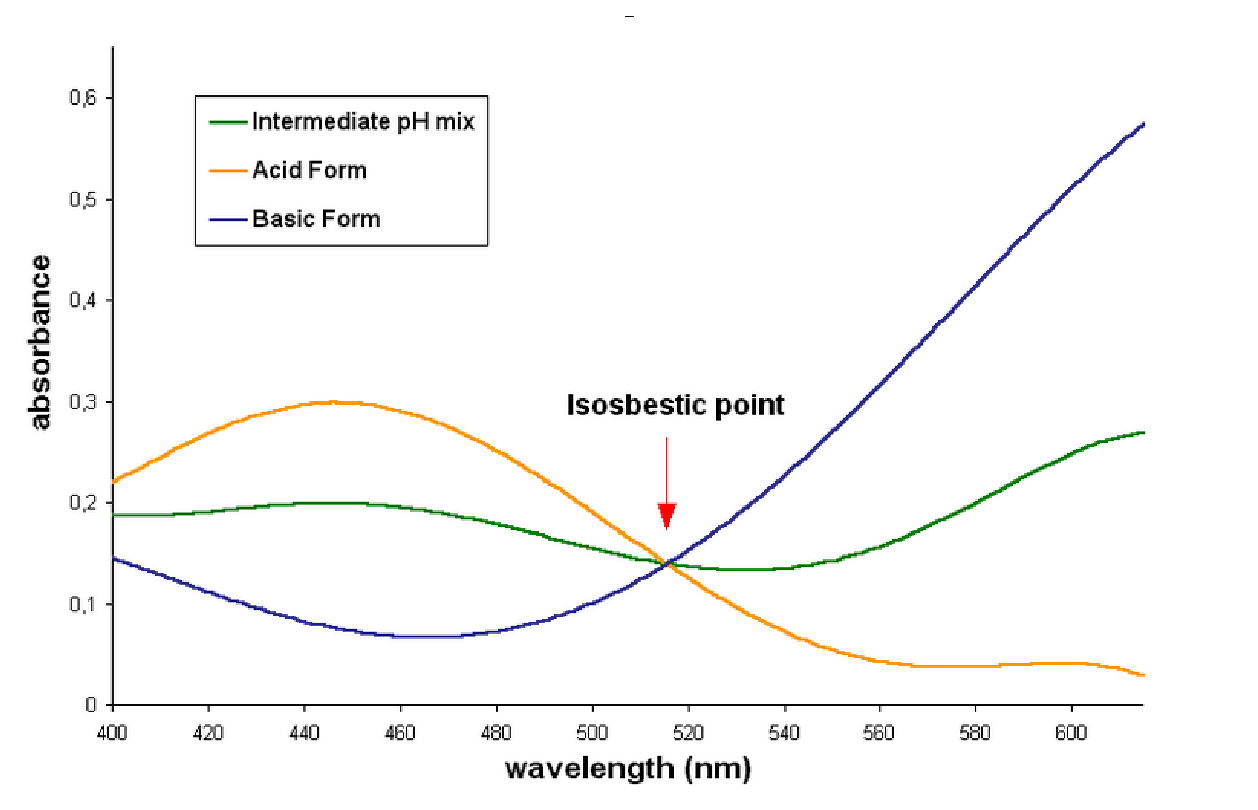
\includegraphics[scale=0.5]{fig4}
\caption{Isosbestic point in UV/VIS absorption spectra. \textit{Note that this figure is just a demonstration and does not correspond to UV/VIS spectra of this experiment}.}
\label{fig4}
\end{center}
\end{figure}

\section{Experimental}

\noindent
\underline{Task overview:}\\

\vspace{0.25cm}

\noindent
\textit{1st laboratory period.} In this series of experiments you will determine $K_a$ from the $pH$ dependence of UV/VIS absorption spectra of aqueous 2-naphthol at 335 nm (with Eqs. (\ref{eq8}), (\ref{eq9}), (\ref{eq10}), (\ref{eq11}) and (\ref{eq12})). Remember that the strongly acidic and basic solutions can be used to calculate the $\epsilon$ values for both ArOH and ArO$^-$. The intermediate values can then be used to calculate $pK_a$ value. Ideally this should give identical result for $pK_a$ at every $pH$ but there will be small variations due to experimental errors. Enter your data in Table \ref{table2}. Note that you will need a blank 3.5'' floppy disk or a USB memory stick for storing your spectra.\\

\vspace{0.25cm}

\noindent
\textit{2nd laboratory period.} Fluorescence spectra of 2-naphthol will be measured under strongly basic and acidic conditions. By overlaying these fluorescence spectra with the corresponding UV/VIS absorption spectra, $\tilde{\nu}_\textnormal{\tiny ArOH}$ and $\tilde{\nu}_{\textnormal{\tiny ArO}^-}$ will be determined as shown in Fig. \ref{fig3}. The $\tilde{\nu}_{00}$ values for ArOH and ArO$^-$ are required in Eq. (\ref{eq6}) to obtain $pK_a^*$. Note that you also need the $pK_a$ value determined in the first laboratory period\\

\vspace{0.25cm}

\noindent
\underline{1st laboratory period:}\\

\noindent
Using the 1.00 mL autopipet, carefully pipet 1.00 mL of the 2.0 $\times$ 10$^{-3}$ M 2-naphthol stock solution into each of five 25 mL volumetric flasks. \textbf{Warning: 2-naphthol is a potential carcinogen}. It is important to use fresh solutions. In an acidic solution, the protonated 2-naphthol predominates. Fill the first flask with 0.02 M HCl. In a basic solution, the deprotonated 2-naphthol predominates. Fill the second flask with 0.02 M NaOH. In the remaining three solutions, a mixture of the protonated and deprotonated forms will be present at intermediate pH levels. These solutions can be obtained by using the provided ammonium chloride buffer solutions as solvents for the three remaining flasks with the following concentrations (NH$_4$OH / NH$_4$Cl): 0.1 M / 0.1 M, 0.1 M / 0.2 M, and 0.2 M / 0.1 M. For the five prepared solutions, the new $\left[\textnormal{ArOH}\right]_0$ concentrations are approximately 8 $\times$ 10$^{-5}$ M.

Absorption spectra of all five solutions should be obtained using the Perkin-Elmer UV/VIS absorption spectrometer (see Table \ref{table1} for spectral range settings). Each spectrum should be saved individually on the computer. Then the five spectra should be overlaid on the computer screen (see Data analysis section). For these spectra a 290 -- 400 nm range can be used. It is essential that the 2-naphthol concentrations are identical (and accurately known) in each case - pipet carefully. Immediately after the spectra are recorded, measure the actual $pH$ of the solution using a properly calibrated $pH$ meter.

Make sure that the spectra obtained as a function of $pH$ satisfy the isosbestic point criterion. If this is not the case, you may need to remake some solutions and retake their spectra. When you are satisfied that the isosbestic point condition is fulfilled for your five solutions, plot your overlaid results on one graph.\\

\vspace{0.25cm}

\noindent
Operation of the Perkin-Elmer Lambda 14 UV/VIS absorption spectrophotometer:

\begin{enumerate}
\item Switch on the Lambda 14.

\item Turn on the computer.

\item Click UVWINLAB.

\item Click SCAN1.MSC.

\item Make sure that the settings are as follows. Scan Tab: WAVELENGTH START = 420 nm, END = 300 nm, DATA INVERVAL 1.00 nm, NUMBER OF CYCLES = 1, ORDINATE MIN = 0.0, ORDINATE MAX = 1.40. Inst. Tab: ORDINATE MODE = A, SCAN SPEED = 240 nm / min, LAMP UV = ON, LAMP VIS = ON, SLIT = 2.0 nm (spectral slit width), SMOOTH = 0 mm. Sample Tab: number of samples = 1, Reults filename = xxx, and Sample Identify = xxx. Here xxx is the filename, for example, your initials and a running index.

%\item Make sure that both cuvette holders are empty, click on AUTOZERO and click OK on the following dialog to record the background spectrum. In this %case the background consists of the natural emission specturm of the light source inside the spectrometer. Note that if you have problems with %background spectrum produced by the solvent, you may have to carry out this step with just the solvent present (i.e., without 2-naphthol). This can be %done by filling the cuvette with the solvent, placing it into the front cuvette holder and clicking on AUTOZERO.

\item If you see a previous spectrum on the screen, select: VIEW $\rightarrow$ REMOVE SPECTRUM.

\item First make sure that both sample holdes in the spectrometer are empty. Click on START. Click OK to measure the background spectrum. After the measurement has finished, put your sample in the front cell holder and click OK.

\item Rescale the spectrum to see it, select: VIEW $\rightarrow$ EXPAND ABSCISSA and VIEW $\rightarrow$ EXPAND ORDINATE.

\item Save the spectrum on a floppy or USB memory stick by selecting: FILE $\rightarrow$ SAVE AS, give the spectrum a unique name and make sure the file type is ASCII (NOT BINARY).

\end{enumerate}

\begin{table}[!htp]
\caption{Summary of the spectral range parameters for UV/VIS and fluorescence measurements.}
\begin{tabular}{l@{\extracolsep{2cm}}l@{\extracolsep{2cm}}l@{\extracolsep{2cm}}l}
 & & & \\
Measurement & Conc. (M) & Range (nm) & Instrument\\
\hline
Absorption & 8 $\times$ 10$^{-5}$ & 300 -- 420 & PE $\lambda$-14\\
Fluorescence ($\lambda_\textit{ex}$ = 311 nm) & 3.2 $\times$ $10^{-6}$ & 320 -- 535 & PE LS50B\\
\end{tabular}
\label{table1}
\end{table}

\noindent
\underline{2nd laboratory period:}\\

\noindent
For the fluorescence spectrometer a more dilute sample must be prepared. Pipet exactly 1 mL of the basic 2-naphthol solution prepared in the first lab period into a 25 mL volumetric flask; dilute to the mark with 0.02 M NaOH. Into a second 25 mL volumetric flask, pipet 1 mL of the acidic solution prepared in the first lab period and dilute to the mark with 0.02 M HCl solution. The 2-naphthol concentration of these solutions should now be 3.2 $\times$ 10$^{-6}$ M. Note that the volumetric dilutions must be performed carefully for the actual concentration must be accurately known.\\

\vspace{0.25cm}

\noindent
Operation of the Perkin Elmer fluorescence spectrometer LS50B:\\

\begin{enumerate}
\item Switch on instrument. Turn on computer.

\item Click on FLWinlab. Close the method dialog by clicking on the cross at the top right corner of the window. Click on the button at the top that has a picture of spectrum in it.

\item Make sure the settings are as follows (with \textit{Setup Parameters} / \textit{Emission Tab} selected): START = 320 nm, END = 500 nm, EXCITATION = 311 nm, EX SLIT = 5.0 nm (spectral slit width), EM SLIT = 5.0 nm (spectral slit width), SCAN SPEED = 240 nm / min. REMEMBER TO SET THE FILENAME AT THE BOTTOM OF THE DIALOG! (it will be saved on the hard disk, the file name should end with .sp extension). Uncheck the AUTO INCREMENT FILENAMES box. If this is not done, the
filenames will get \#\textit{xx} (\textit{xx} = number) tagged on them. Be sure to change the filename for each scan.

\item Use a \textbf{four clear-sided quartz cell}. Do not leave fingerprints on it.

\item Click green ``traffic light''button (top-left corner).

\item Click the autoexpand buttons (above the spectrum, red arrows on the buttons).

\item Close the Scan window by choosing FILE $\rightarrow$ EXIT. It is not necessary to save the method -- the spectrum was saved automatically.

\item \textbf{Make sure that your spectra are not clipped}. If the top of the peaks are flat (i.e., clipped), 
you will need to decrease the EM and EX slits (see above) or dilute your samples.

\item To save the spectrum in ASCII format on your floppy or USB memory stick, select (in FL WinLab window) FILE $\rightarrow$ OPEN. Type in the spectrum filename (from step 3.) in ``Filename:'' text box. Note that your file may not appear in the list of files (program bug) and you have to manually type in the file name. The spectrum should appear on the screen. If you get multiple spectra overlaid, then you should remove the unwanted spectra with VIEW $\rightarrow$ REMOVE CURVE. Make sure that the graph that you want to save is active (by clicking on the graph name below the spectrum). Finally, choose FILE $\rightarrow$ SAVE AS, choose the file type as ASCII (not BINARY), double click on a: drive on the right, you may change the filename if you like, and press OK.

\end{enumerate}

\section{Data analysis}

\begin{itemize}
\item Determine the isosbestic point for the five UV/VIS absorption spectra.\\

\begin{itemize}
\item[--] Insert your data floppy into the drive or your USB stick into a USB port.

\item[--] Use the qtiplot program to produce an overlay plot of the absorption spectra. Each spectrum can be read in by using the ``File $\rightarrow$ Import $\rightarrow$ Import ASCII...''. Click on the ``Advanced'' button and make sure that you have Separator selected as TAB (X and Y values separated by tabulators) and Ignore first is set to 86 (skip this many first lines in the file). Click on ``Open'' to read in the spectrum. A new table for each spectrum will appear on the screen. 

\item[--] Plot the first specturm by selecting the Y column in the table (click on the column heading with mouse so that it becomes highlighted) and then choose ``Plot $\rightarrow$ Line''. To add the rest of spectra to the graph, click on the graph and select ``Graph $\rightarrow$ Add/Remove Curve...'' from the top menus. For each table, click on it and press the right arrow with mouse. The new spectra will appear on the screen. You can edit the axis etc. by double clicking on them.

\item[--] Print a copy of the graph by selecting File $\rightarrow$ Print. Mark the isosbestic point in the graph and include a copy of the printout with your laboratory report.

\item[--] Exit qtiplot. If you want to take out your floppy or USB stick, right click on the floppy icon on the desktop and choose ``Unmount volume''.

\end{itemize}

\item Determine $\epsilon$ values and $pK_a$ at 335 nm. Use the following table to present your data.\\

\begin{table}[!htp]
\caption{Table of experimental results from the UV/VIS measurements.}
\begin{tabular}{|l|l|l|l|l|l|}
\hline
Solution \# & Solution $pH$ & $A$ at 335 nm & [ArOH] & [ArO$^-$] & Calculated $K_a$\\
\hline
1 & \hspace{2cm} & \hspace{2cm} & \hspace{2cm} & \hspace{2cm} & N/A\\
\hline
2 & \hspace{2cm} & \hspace{2cm} & \hspace{2cm} & \hspace{2cm} & \hspace{2cm}\\
\hline
3 & \hspace{2cm} & \hspace{2cm} & \hspace{2cm} & \hspace{2cm} & \hspace{2cm}\\
\hline
4 & \hspace{2cm} & \hspace{2cm} & \hspace{2cm} & \hspace{2cm} & \hspace{2cm}\\
\hline
5 & \hspace{2cm} & \hspace{2cm} & \hspace{2cm} & \hspace{2cm} & N/A\\
\hline
\end{tabular}
\label{table2}
\end{table}

\item Overlay of the UV/VIS and fluorescence spectra to obtain the $\tilde{\nu}_{00}$ values. This must be done for both acidic and basic cases.\\

\begin{itemize}
\item[--] Insert your data floppy into the floppy drive or your USB memory stick into USB port.

\item[--] Use the qtiplot to overlay the absorption and fluorescence spectra. Import the spectra the same way as you did when determining the isobestic point. Use ``Graph $\rightarrow$ Line'' to plot the first spectrum and then add the second spectrum by first selecting the graph with the mouse and then choosing ``Graph $\rightarrow$ Add/Remove Curve...'' (i.e., just like was done when determining the isobestic point).

\item[--] Fix the baseline for each spectra. Look at the last row of the table (i.e., the row with the largest wavelength). Write down the Y column value there. Select the Y coloumn and choose ``Table $\rightarrow$ Set Column Values...'' and write the following expression in the large input box: col(``2'') $-$ XXX, where XXX is the number you wrote down. You should see now that the baseline of the spectrum is at zero.

\item[--] Normalize both spectra by selecting their Y columns and choosing ``Analyze $\rightarrow$ Normalize $\rightarrow$ Columns''. Their maximum values should now be one.

\item[--] Use ``Data $\rightarrow$ Data reader'' to record the wavelength where the two spectra cross. Convert the value to wavenumbers to obtain $\tilde{\nu}_{00}$.

\item[--] You can set the axis labels etc. by double clicking on the corresponding areas on the graph. Indicate the absorption/fluorescence spectrum corrossing point by drawing an arrow pointing at it (use ``Graph $\rightarrow$ Add arrow'' and draw the arrow with mouse). Finally print a copy of the overlaid spectra.

\item[--] Exit the program by File $\rightarrow$ Exit. If you want to take out your floppy or USB memory stick, right click on the floppy icon on the desktop and choose ``Unmount volume''.

\end{itemize}
\end{itemize}

\section{Error analysis}

Calculate the error in $pK_a$ by using the standard deviation of the three measured points:

\begin{equation}
\label{eq13}
\delta pK_a = \sqrt{\frac{\sum\limits_{i=1}^{3}\left(\overline{pK_a} - pK_a(i)\right)^2}{3}}
\end{equation}

\noindent
where $pK_a(i)$ is the $pK_a$ value obtained from the $i$th run and the overbar denotes an average value. Note that in this case we would like to have more than three points in order to get a better error estimate. The error in $\Delta\tilde{\nu}$ (see Eq. (\ref{eq6})) should be obtained by estimating the accuracy by which the spectra can be read. The total error in $pK_a^*$ is then given by:

\begin{equation}
\label{eq14}
\delta pK_a^* = \sqrt{\left(\frac{\partial pK_a^*}{\partial pK_a}\right)^2 \times \left(\delta pK_a\right)^2 + \left(\frac{\partial pK_a^*}{\partial\Delta\tilde{\nu}}\right)^2 \times \left(\delta\Delta\tilde{\nu}\right)^2}
\end{equation}

In order to use this equation, partial derivatives for Eq. (\ref{eq6}) must be calculated (exercise).

\section{Written laboratory report}

Follow the general instructions for written laboratory reports. In addition, include the requested data in the following section:\\

\noindent
\textit{Results.} This section must include the values for $pK_a$ and $pK_a^*$. Find the literature values for these quantities \cite{LOEFROTH}. Compare the values of $pK_a$ and $pK_a^*$, and explain what the difference in acidity constants tells us about $\Delta H$ and $\Delta H^*$ (see Fig. \ref{fig2}). Carry out error analysis using the method given in the data analysis section and give a complete expression for Eq. (\ref{eq14}) where the partial derivatives have been written. Remember to include copies of the graphs prepared in the data analysis section.\\

\noindent
\textbf{Acknowledgment:} This laboratory exercise was adapted from that given in Ref. \cite{MCBANE}.

\section{References}

\vspace{-1cm}

\bibliography{../references}

\end{document}
